\section*{Molekylefysik}
\begin{table*}[h!]
    \centering
    \begin{tabular}{c|c c c c c c c c c c|}
\hline &H&He&Li&Be&B&C&N&O&F&Ne\\\hline
$1s$&-13,6&-25,0 & -67,4 & -128,8&-209,4&-308,5&-426,3&-562,7&-717,9&-891,7\\
$2s$&&&-5,3&-8,4&-13,5&-19,4&-26,2&-34,0&-42,8&-52,5\\
$2p$&&&&&-8,4&-11,1&-13,8&-16,8&-19,9&-23,1\\\hline
    \end{tabular}
    \caption{Energierne for de laveste atomorbitaler i de første ti grundstoffer.}
    \label{amo:tab:aoenergi}
\end{table*}
%
\begin{opgave}{Diatomare molekyler}{1}
\opg På figur \ref{k-fig:diatomar} i kompendiet er tegnet molekyleorbitaldiagrammer for O$_2$ og N$_2$. Gør det samme for C$_2$, F$_2$ og Ne$_2$.
\opg Hvad er bindingsordenen af de fem molekyler?
\opg Hvilket vil I forvente er mest stabilt?
\opg Hvilket forventer I er mest ustabilt?
\opg Hvor mange af molekylerne har uparrede elektroner, og er dermed magnetiske?
\end{opgave}
%
\begin{opgave}{Vand}{2}
Vi vil her konstruere en model for vandmolekylet ud fra et iltatom og et brintmolekyle. Vand består af et iltatom og to brintatomer, og det har form som et $V$. I vores model dannes vand ved at bevæge et brintmolekyle ind imod et iltatom, hvorefter brintmolekylet strækkes og bliver til de to grene af V'et.\\
Bemærk at ikke alle orbitaler indgår i bindingen.
\opg Skitser molekyleorbitalerne for brint.
\opg Skitser atomorbitalerne for ilt.
\opg Hvilke af orbitalerne overlapper?
\opg Opstil et molekyleorbitaldiagram.
\opg Hvilke af de resulterende orbitaler er bindende, antibindende eller ikke bindende?
\opg Hvad er bindingsordenen af molekylet?
\end{opgave}
%
\begin{opgave}{Benzen}{3}
Som meget kort nævnt i kompendiet kan $\pi$-bindinger medføre at elektronerne i et molekyle er delokaliserede, dvs. det er muligt at finde dem inden for et stort område (på molekylær skala). Dette sker blandt andet i benzenmolekylet. Benzen består af seks kulstof atomer i en sekskant, med et brintatom bundet til hver. $\sigma$-bindingerne i Benzen er ikke noget specielt, så vi vil udelukkende beskæftige os med $\pi$-bindingerne.
Kulstof atomernes $p_z$-orbitaler, der danner $\pi$-bindingerne, er ikke egentilstande. Kulstof atomerne rundt langs ringen gives numre fra 1 til 6. Det giver orbitalerne $p_1$ til $p_6$. 
\opg Hvad er $p_7$? \\
Det viser sig at Hamiltonoperatoren på en af $p$ orbitalerne giver:
$$
\op H p_j = \alpha p_j+\beta p_{j+1}+\beta p_{j-1}
$$
Her er $\alpha$ og $\beta$ konstanter.
En bølgefunktion med mange knudeflader (knudepunkter i 3 dimensioner) vil normalt have højere energi end en med få knude flader.
\opg Opstil og skitser en bølgefunktion $1\pi$, ud fra $p_z$-orbitalerne for kulstof, med så få knudeflader som muligt.
\opg Opstil og skitser en bølgefunktion $6\pi$ med så mange knudeflader som muligt.
\opg Afgør om $1\pi$ og $6\pi$ er egenfunktioner for $\op H$ og find deres energi.
\opg $\alpha$ er en positiv konstant, så hvad er fortegnet på $\beta$?\\ 
De resterende bølgefunktioner er:
\begin{align*}
2\pi &= \frac{1}{2\sqrt{3}}(2p_1+p_2-p_3-2p_4-p_5+p_6)\\
3\pi &= \frac{1}{2}(p_2+p_3-p_5-p_6)\\
4\pi &= \frac{1}{2\sqrt{3}}(2p_1-p_2-p_3+2p_4-p_5-p_6)\\
5\pi &= \frac{1}{2}(p_2-p_3+p_5-p_6)
\end{align*}
\opg Skitser også disse bølgefunktioner og find deres energi.
\opg Lav et molekyleorbitaldiagram for $\pi$-systemet for Benzen.
\end{opgave}

\begin{figure}[t]
	\centering
	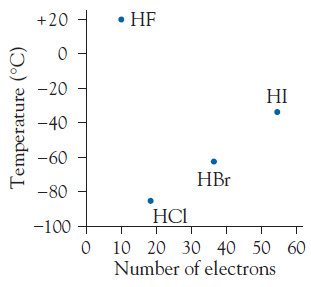
\includegraphics[width=\columnwidth]{Atom-ogMolekylefysik/billeder/HX-kogepunkt.png}
	\caption{Kogepunkterne for hydrogenhaliderne.} %Kilde: DIC.}
	\label{fig:HX-kogepunkt}
\end{figure}
\begin{opgave}{Halogener og hydrogenbindinger}{3}
Et vigtigt resultat der lægger grunden for en masse kemi, er at elektronkonfigurationer, hvor den yderste $s$- og $p$-orbital er fyldte er særligt stabile, hvilket leder til, hvad der i kemi kaldes "oktetreglen". Dette resultat har nogle interessante konsekvenser, der her vil undersøges.
\opg Hvilken elektronkonfiguration har flour, $F$, der er grundstof nummer 9?
\opg Flour står i 17. gruppe, der også kaldes halogenerne, som alle er karakteriseret ved at have samme elektronkonfiguration i deres yderste $s$- og $p$-orbitaler. Hvorfor er denne konfiguration speciel?
\opg Ligesom hydrogen samler halogenerne sig i molekyler på formen $\mathrm{X}_2$, hvor X er et vilkårlig halogen. Blandes en halogengas med hydrogengas forekommer følgende reaktion
\begin{align*}
	\mathrm{H}_2(g) + \mathrm{X}_2(g) \rightarrow 2 \mathrm{HX}(g)
\end{align*}
Forklar med et molekylorbitaldiagram, hvorfor HF er mere stabilt end $\mathrm{H}_2$ og $\mathrm{F}_2$.
\opg Hvilke atomorbitaler danner bindingen i HF, og hvilken type er det?
\opg I eksemplet med $\mathrm{H}_2$ er de to atomer ens, hvorfor orbitalen er symmetrisk omkring en akse midt imellem de to atomer. Hvis de to atomer er forskellige, eller det ikke er samme orbitaler der binder, er dette ikke nødvendigvis sandt. Hvorfor er molekylorbitalen for HF forskudt og imod hvilket atom?
\opg Denne forskydning giver HF et dipolmoment\footnote{Mere præcist kan det siges, at der er størst sandsynlighed for at de bindende elektroner befinder sig tættere på det ene atom end det andet, og ikke omvendt eller ligeligt fordelt. Det betyder at forventningsværdien, $\expect{\v{r}}$, vil være forskudt mod det ene atom. Det siges derfor ladningen i gennemsnit samler sig hos dette atom, som så er partielt negativt ladet, mens det andet er partielt positivt ladet.}, hvilket i denne sammenhæng fint kan tænkes som en ladningsforskydning, hvor alle elektronerne befinder sig tættere på det ene atom end det andet. Forklar hvorfor det betyder, at et HF-molekyle tiltrækkes af de andre, hvilket kaldes at de danner hydrogenbindinger?
\opg HF er det eneste af hydrogenhaliderne, HX, der kan danne hydrogenbindinger, hvilket kan ses på deres kogepunkter, figur \ref{fig:HX-kogepunkt}. Hvorfor det? \\ \\
Netop denne forskel gør flussyre, der er en vandig opløsning af HF, speciel. Den er i modsætning til de andre hydrogenhalider i stand til at opløse glas, hvorfor den ikke er så let at opbevare. Derudover kan den trænge igennem huden og opløse kroppen indefra, hvorfor eksempelvis saltsyre, HCl, oftere benyttes i laboratoriet.
\end{opgave}